\chapter{実現方法}\label{chap:method}

ARマーカーを用いずに原点を調整する手法として、マップ画像を用いて手動で調整する手法を提案する。


\section{内部情報の取得}

ロボットの内部情報の取得には、ROS#を用いた。
ROS#とは、Unity上でROSを利用できるようにするパケージで、UnityとROSでデータの通信が可能になる。
また、取得したデータは数値データであるため、可視化の作業もROS#を用いて行っている。
図\ref{VisRosUni}は、RvizとUnityでセンサーの可視化を行った様子である。
UnityでもRvizと同じような可視化結果が出力できていることがわかる。


\begin{figure}[H]
  \begin{minipage}[b]{0.45\linewidth}
    \centering
    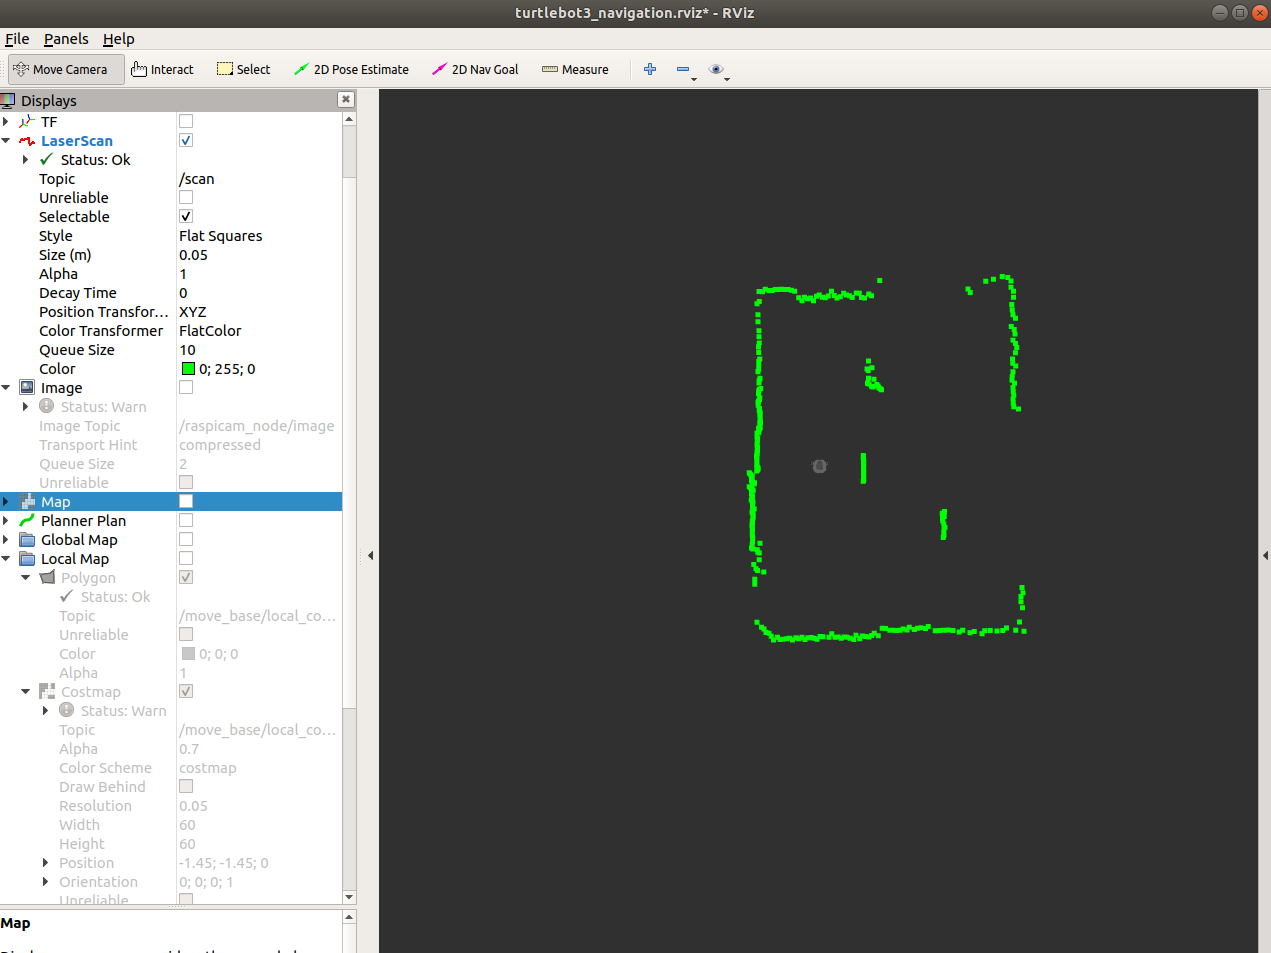
\includegraphics[keepaspectratio, width=.9\hsize]{figs/Rviz_Lidar.png}
    \subcaption{Rviz上での可視化}
  \end{minipage}
  \begin{minipage}[b]{0.45\linewidth}
    \centering
    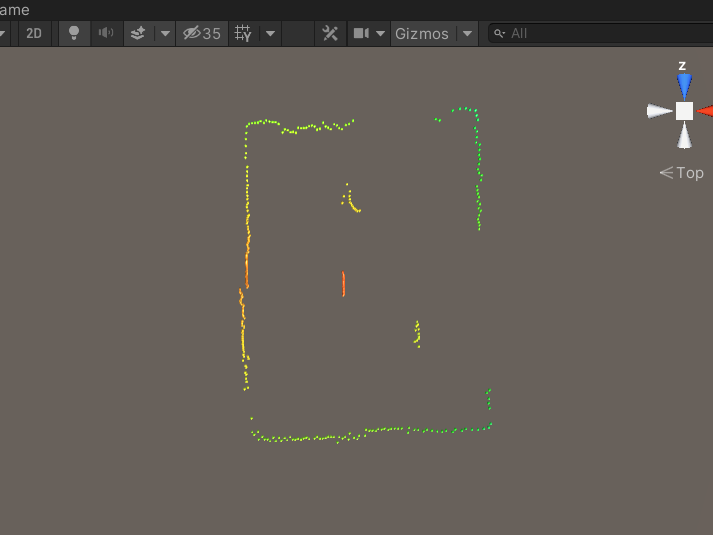
\includegraphics[keepaspectratio, width=.9\hsize]{figs/Unity_Lidar.png}
    \subcaption{Unity上での可視化}
  \end{minipage}
  \caption{データの可視化}\label{VisRosUni}
\end{figure}


\section{ARで可視化}

ARで可視化には、ARcoreを利用した。
ARcoreとは、Googleが提供するARプラットフォームであり、端末のトラッキングやオブジェクトの配置ができる。
トラッキングには、Visual Odometryという画像の特徴点から端末の移動量を推定する技術が利用されている。


\section{ARで可視化}

